\mychapter{Experiments}\label{sec:exp}
We conduct experiments to compare the following two methods to solve \eqref{eq:reMF}.
\begin{itemize}
\item Newton method described in Section~\ref{sec:NewtonMin}.
\item Alternating Newton method \citep{WSC18a} described in Section~\ref{sec:NewtonFM}.
\end{itemize}
\mysection{Experimental Settings}
\begin{table}[H]
\caption{Statistics and parameters for each data set.}
\centering
\begin{tabular}{r|rrr}
Data Set   & \tt movielens10m & \tt netflix  & \tt movielens1m\\ \hline
$M$          & 71,567        & 2,649,429  & 6,040\\
$N$          & 65,133        & 17,770    & 3,952\\
\#Training & 9,301,274      & 99,072,112 & *\\
\#Test     & 698,780       & 1,408,395 & *\\
$d$				& 40					& 20			& 40
\end{tabular}
\label{tab:dataset}
\end{table}
We consider data sets listed in Table \ref{tab:dataset}. For both methods, every element of initial $U$ and $V$ is randomly drawn from the interval $[-0.1/\sqrt{d},{0.1}/\sqrt{d}]$. 
\par For the CG procedure, we set $\eta=0.3$ as the stopping tolerance. Note that we consider the same $\eta$ for the CG procedure in both Algorithms \ref{alg:CG} and \ref{alg:Pcg}. For the line search procedure, we set $\beta=0.5$ as the ratio to decrease the step size and $\nu=0.1$ for the sufficient decrease condition \eqref{eq:LineSearchRule}. For the latent dimension, we use $d$ listed in Table \ref{tab:dataset}.

\begin{figure*}[tb]
        \centering
        \begin{subfigure}[b]{0.32\textwidth}
                \centering
                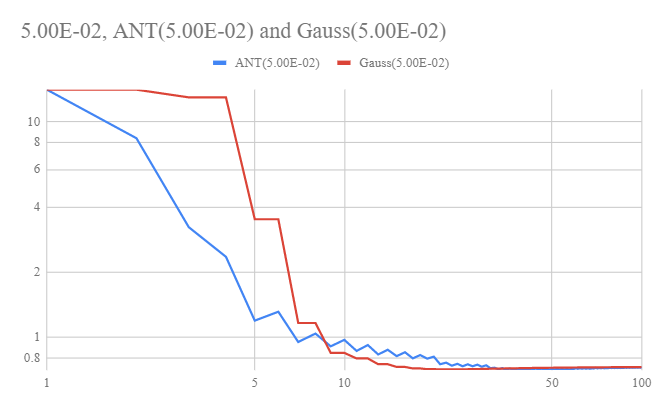
\includegraphics[width=\textwidth]{{figures/ml1m_5e-2_valoss_iter_.png}}
                \caption{ml-1m.5e-2}
        \end{subfigure}
        \begin{subfigure}[b]{0.32\textwidth}
                \centering
                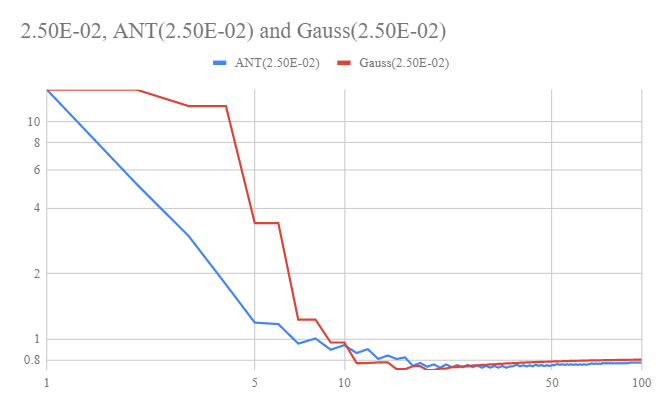
\includegraphics[width=\textwidth]{{figures/ml1m_2point5e-2_valoss_iter.png}}
                \caption{ml-1m.2.5e-2}
        \end{subfigure}
        \begin{subfigure}[b]{0.32\textwidth}
                \centering
                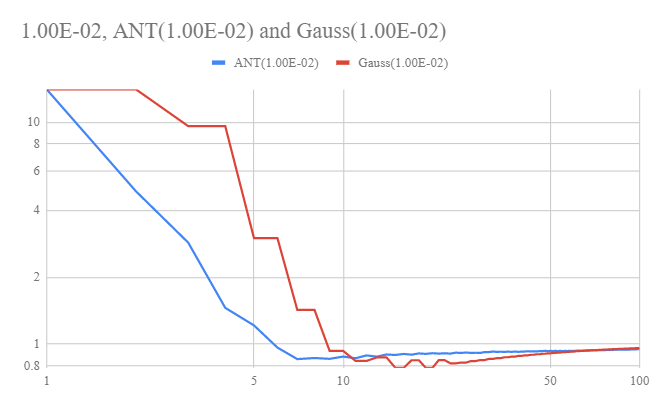
\includegraphics[width=\textwidth]{{figures/ml1m_1e-2_valoss_iter.png}}
                \caption{ml-1m.1e-2}
        \end{subfigure}
        \begin{subfigure}[b]{0.32\textwidth}
                \centering
                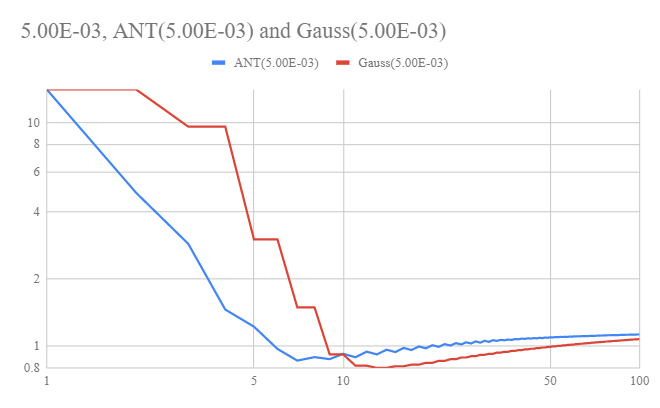
\includegraphics[width=\textwidth]{{figures/ml1m_5e-3_valoss_iter_.png}}
                \caption{ml-1m.5e-3}
        \end{subfigure}
        \begin{subfigure}[b]{0.32\textwidth}
                \centering
                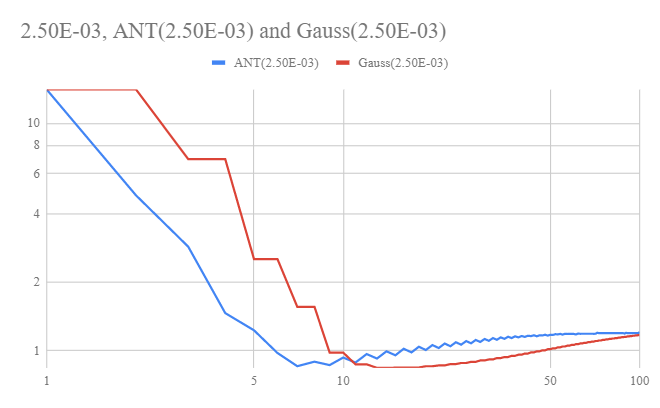
\includegraphics[width=\textwidth]{{figures/ml1m_2point5e-3_valoss_iter.png}}
                \caption{ml-1m.2.5e-3}
        \end{subfigure}
        \begin{subfigure}[b]{0.32\textwidth}
                \centering
                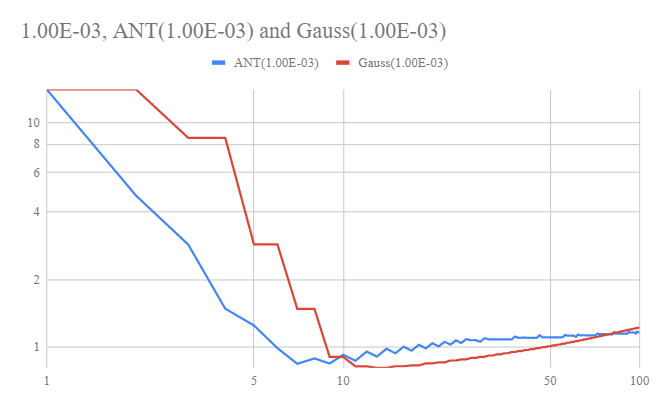
\includegraphics[width=\textwidth]{{figures/ml1m_1e-3_valoss_iter.png}}
                \caption{ml-1m.1e-3}
        \end{subfigure}    
        \begin{subfigure}[b]{0.32\textwidth}
                \centering
                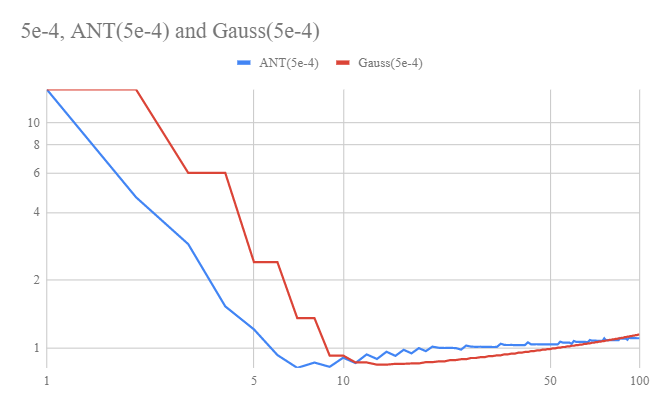
\includegraphics[width=\textwidth]{{figures/ml1m_5e-4_valoss_iter.png}}
                \caption{ml-1m.5e-4}
        \end{subfigure}
        \begin{subfigure}[b]{0.32\textwidth}
                \centering
                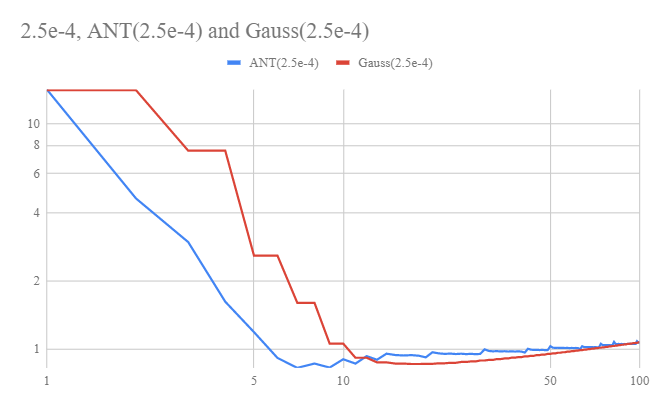
\includegraphics[width=\textwidth]{{figures/ml1m_2point5e-4_valoss_iter.png}}
                \caption{ml-1m.2.5e-4}
        \end{subfigure}
        \begin{subfigure}[b]{0.32\textwidth}
                \centering
                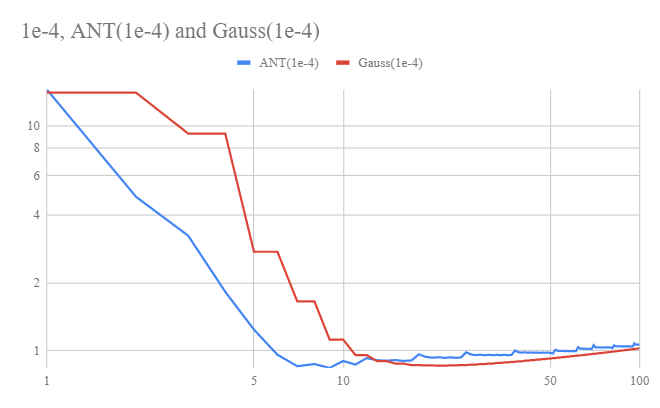
\includegraphics[width=\textwidth]{{figures/ml1m_1e-4_valoss_iter.png}}
                \caption{ml-1m.1e-4}
        \end{subfigure}    
        \begin{subfigure}[b]{0.32\textwidth}
                \centering
                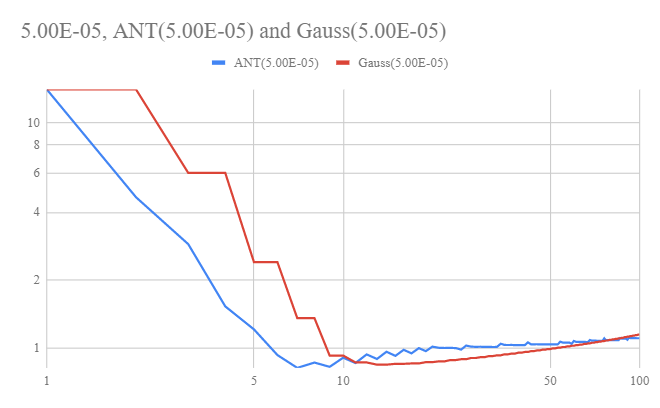
\includegraphics[width=\textwidth]{{figures/ml1m_5e-5_valoss_iter.png}}
                \caption{ml-1m.5e-5}
        \end{subfigure}
        \begin{subfigure}[b]{0.32\textwidth}
                \centering
                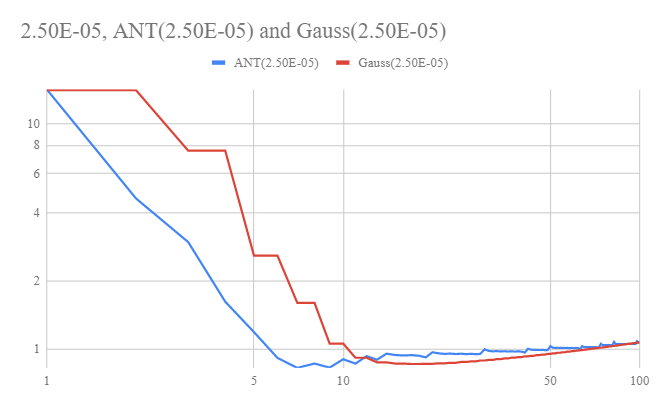
\includegraphics[width=\textwidth]{{figures/ml1m_2point5e-5_valoss_iter.png}}
                \caption{ml-1m.2.5e-5}
        \end{subfigure}
        \begin{subfigure}[b]{0.32\textwidth}
                \centering
                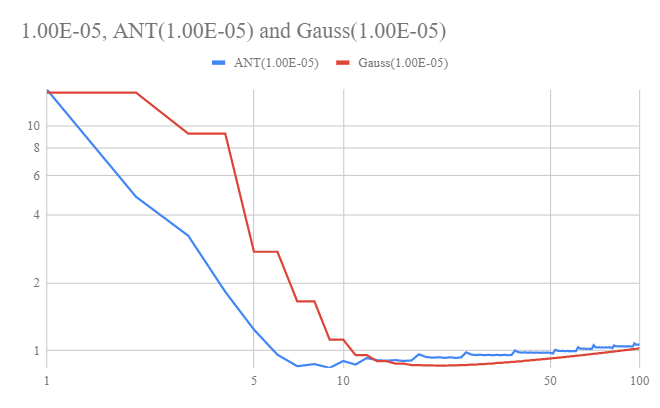
\includegraphics[width=\textwidth]{{figures/ml1m_1e-5_valoss_iter.png}}
                \caption{ml-1m.1e-5}
        \end{subfigure} 
        \begin{subfigure}[b]{0.32\textwidth}
                \centering
                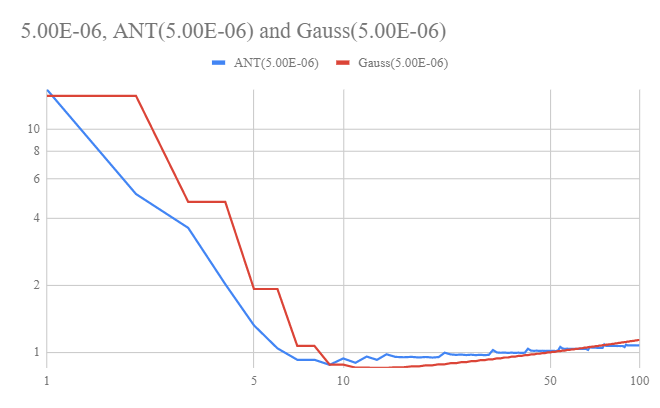
\includegraphics[width=\textwidth]{{figures/ml1m_5e-6_valoss_iter.png}}
                \caption{ml-1m.5e-6}
        \end{subfigure}
        \begin{subfigure}[b]{0.32\textwidth}
                \centering
                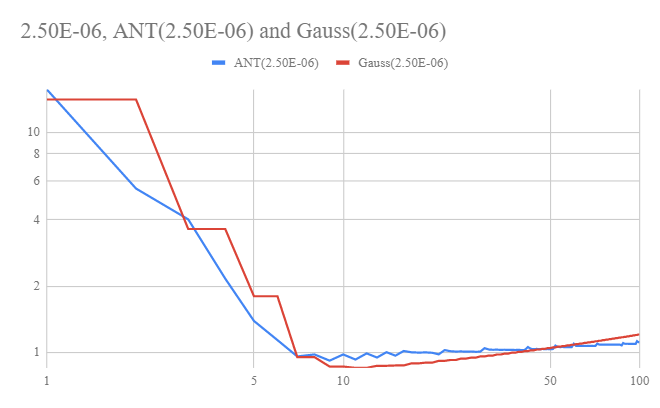
\includegraphics[width=\textwidth]{{figures/ml1m_2point5e-6_valoss_iter.png}}
                \caption{ml-1m.2.5e-6}
        \end{subfigure}
        \begin{subfigure}[b]{0.32\textwidth}
                \centering
                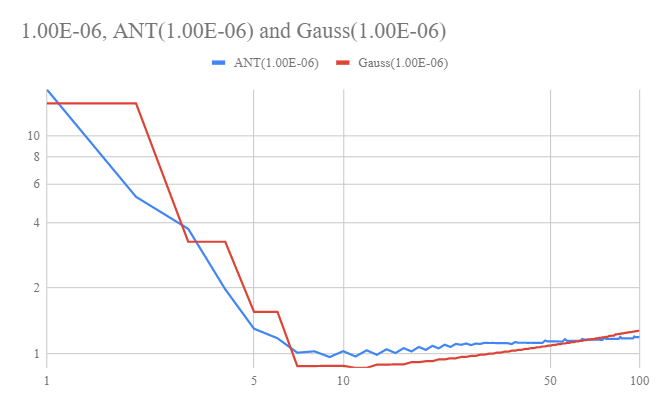
\includegraphics[width=\textwidth]{{figures/ml1m_1e-6_valoss_iter.png}}
                \caption{ml-1m.1e-6}
        \end{subfigure}        
        \begin{subfigure}[b]{0.32\textwidth}
                \centering
                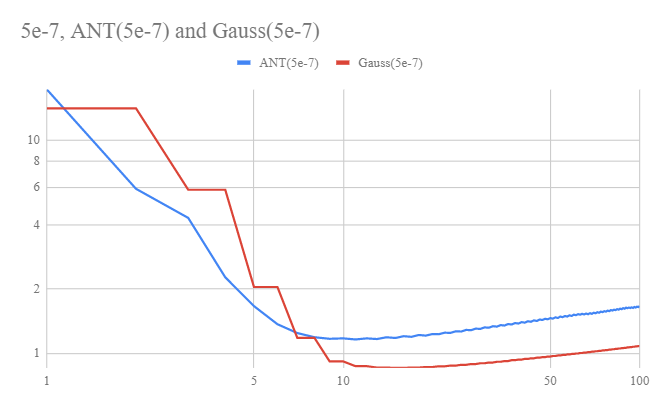
\includegraphics[width=\textwidth]{{figures/ml1m_5e-7_valoss_iter.png}}
                \caption{ml-1m.5e-7}
        \end{subfigure}
        \begin{subfigure}[b]{0.32\textwidth}
                \centering
                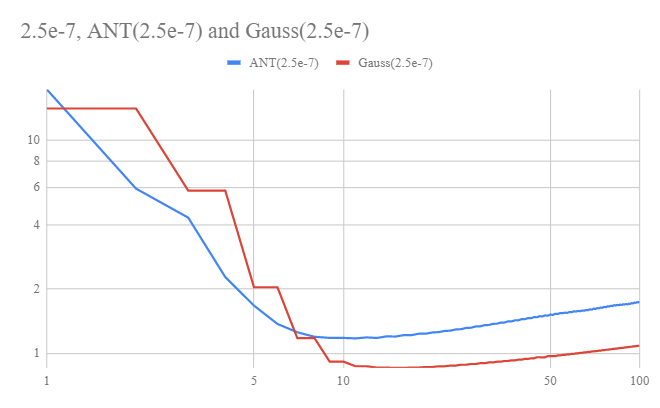
\includegraphics[width=\textwidth]{{figures/ml1m_2point5e-7_valoss_iter.png}}
                \caption{ml-1m.2.5e-7}
        \end{subfigure}
        \begin{subfigure}[b]{0.32\textwidth}
                \centering
                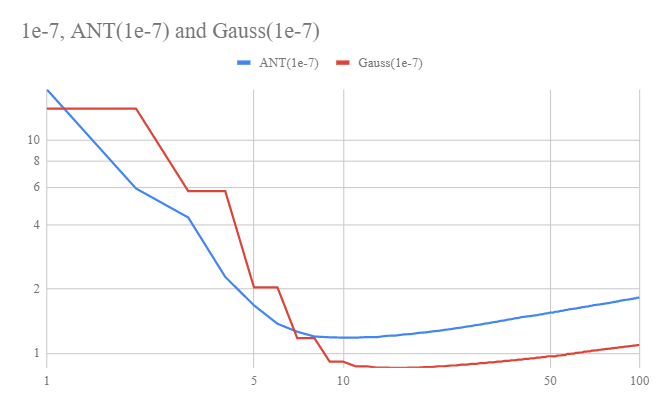
\includegraphics[width=\textwidth]{{figures/ml1m_1e-7_valoss_iter.png}}
                \caption{ml-1m.1e-7}
        \end{subfigure} 
        \caption{A comparison on the va-loss of different methods. ANT is worse than Gauss among smaller $\lambda$.
        The $x$-axis is the iteration,
        while the $y$-axis is the va-loss.}\label{fig:ant_gauss_valoss_iter_}
\end{figure*}

\begin{figure*}[tb]
        \centering
        \begin{subfigure}[b]{0.32\textwidth}
                \centering
                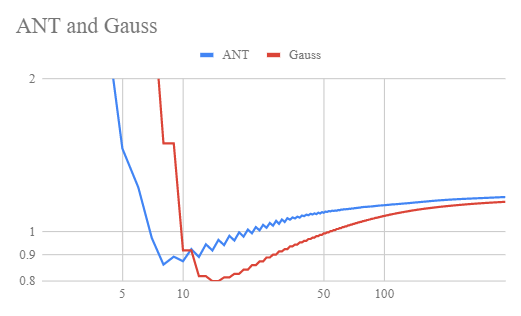
\includegraphics[width=\textwidth]{{figures/ml1m_5e-3_valoss_iter.png}}
                \caption{ml-1m.5e-3}
        \end{subfigure}
        \begin{subfigure}[b]{0.32\textwidth}
                \centering
                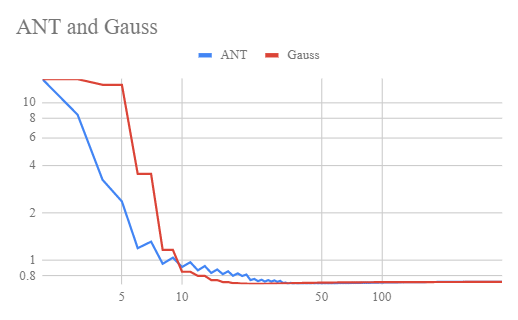
\includegraphics[width=\textwidth]{{figures/ml1m_5e-2_valoss_iter.png}}
                \caption{ml-1m.5e-2}
        \end{subfigure}
        \begin{subfigure}[b]{0.32\textwidth}
                \centering
                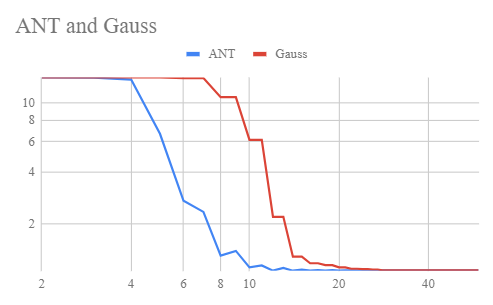
\includegraphics[width=\textwidth]{{figures/ml1m_5e-1_valoss_iter.png}}
                \caption{ml-1m.5e-1}
        \end{subfigure}
        \begin{subfigure}[b]{0.32\textwidth}
                \centering
                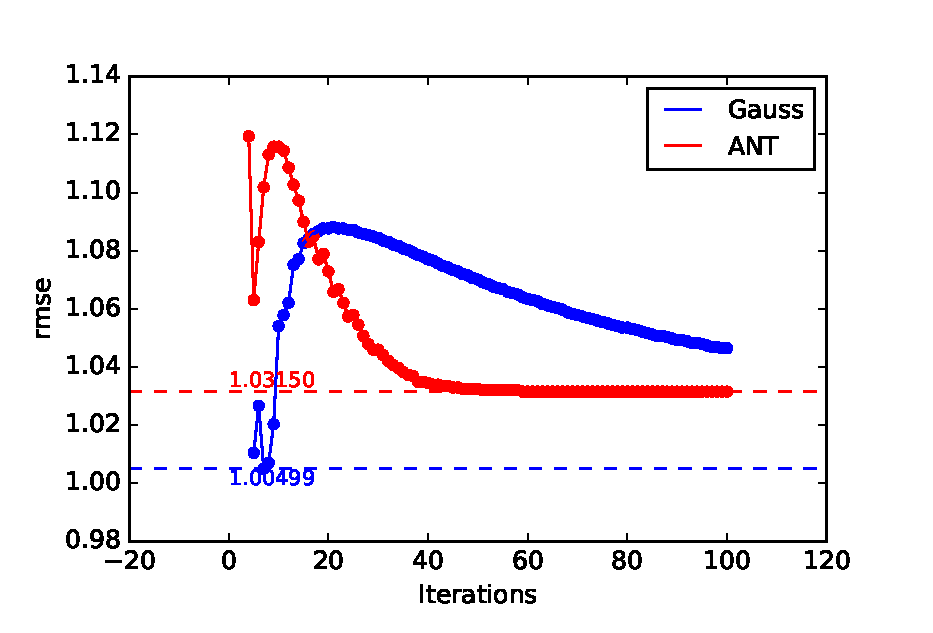
\includegraphics[width=\textwidth]{{figures/ml.0.005.rmse.iter.eps}}
                \caption{ml-10m.5e-3}
        \end{subfigure}
        \begin{subfigure}[b]{0.32\textwidth}
                \centering
                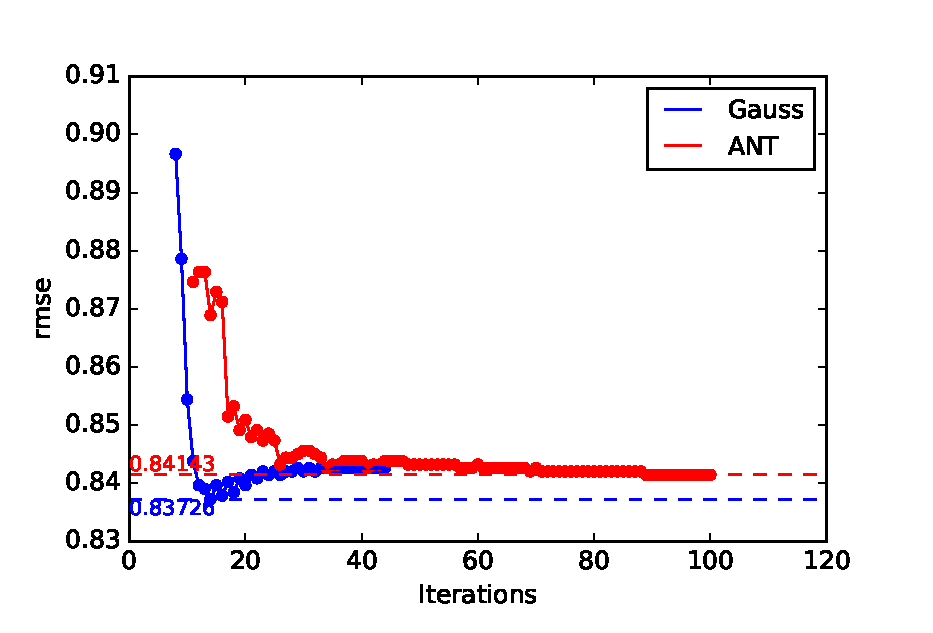
\includegraphics[width=\textwidth]{{figures/ml.0.05.rmse.iter.eps}}
                \caption{ml-10m.5e-2}
        \end{subfigure}
        \begin{subfigure}[b]{0.32\textwidth}
                \centering
                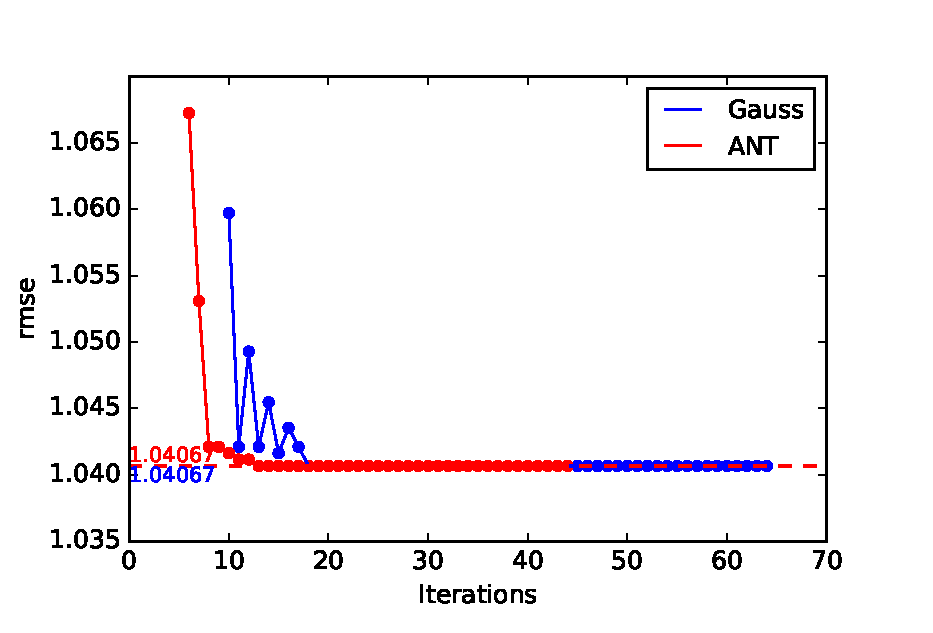
\includegraphics[width=\textwidth]{{figures/ml.0.5.rmse.iter.eps}}
                \caption{ml-10m.5e-1}
        \end{subfigure}
        \begin{subfigure}[b]{0.32\textwidth}
                \centering
                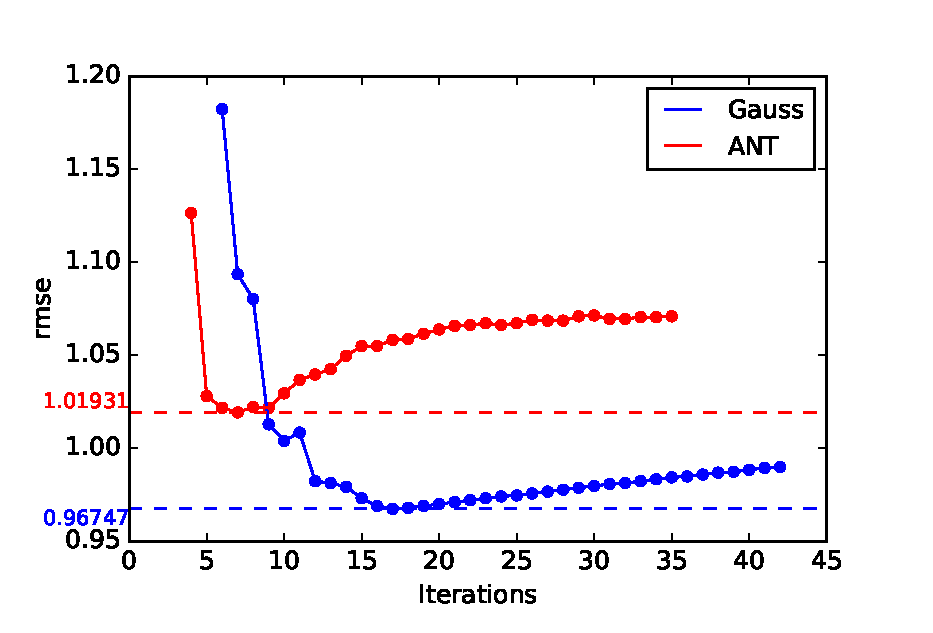
\includegraphics[width=\textwidth]{{figures/nf.0.005.rmse.iter.eps}}
                \caption{nf.5e-3}
        \end{subfigure}
        \begin{subfigure}[b]{0.32\textwidth}
                \centering
                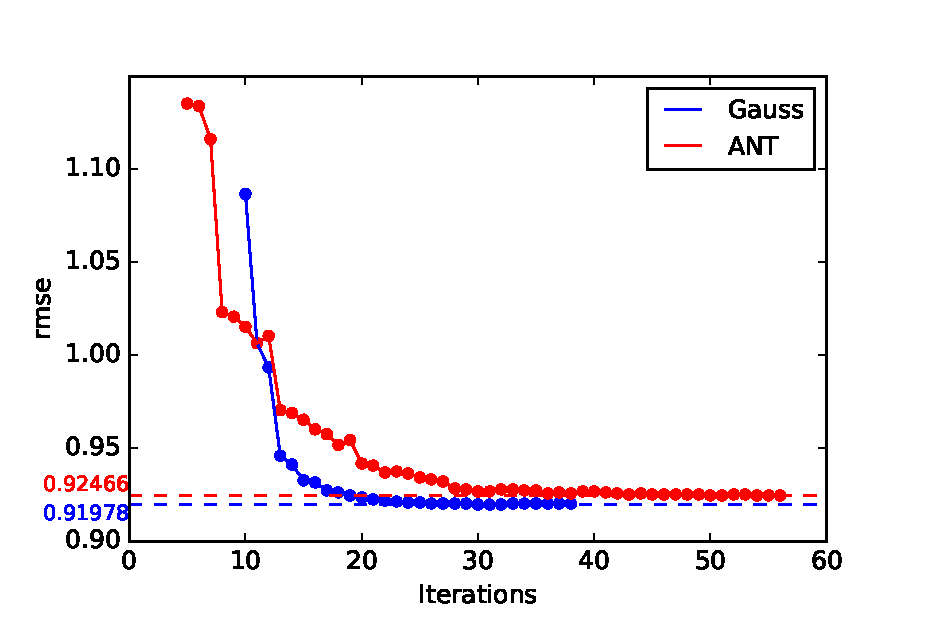
\includegraphics[width=\textwidth]{{figures/nf.0.05.rmse.iter.eps}}
                \caption{nf.5e-2}
        \end{subfigure}
        \begin{subfigure}[b]{0.32\textwidth}
                \centering
                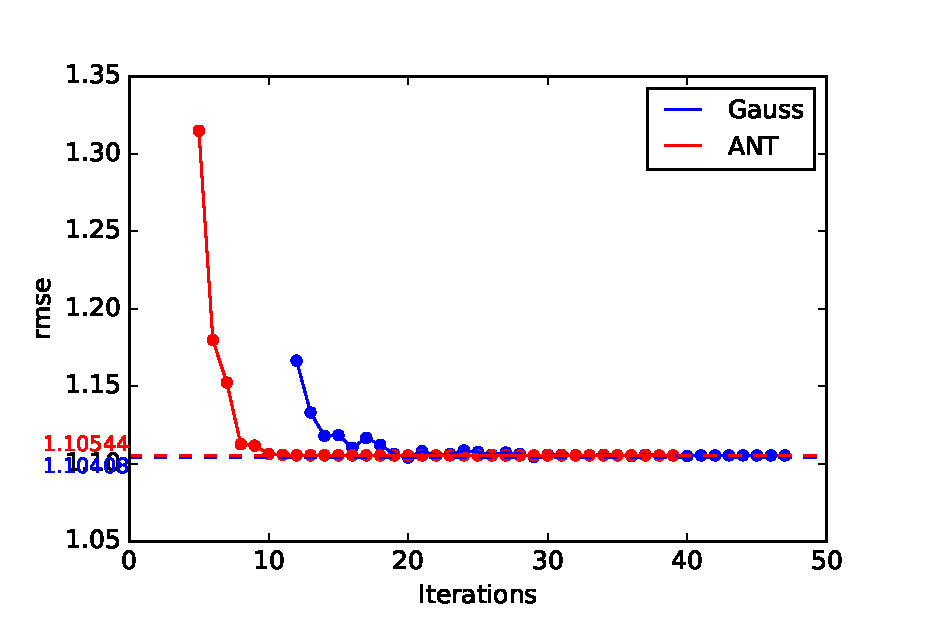
\includegraphics[width=\textwidth]{{figures/nf.0.5.rmse.iter.eps}}
                \caption{nf.5e-1}
        \end{subfigure}
        \caption{A comparison on the va-loss of different methods.
        The $x$-axis is the iteration,
        while the $y$-axis is the va-loss.}\label{fig:ant_gauss_valoss_iter}
\end{figure*}

\begin{figure*}[tb]
        \centering
        \begin{subfigure}[b]{0.9\textwidth}
                \centering
                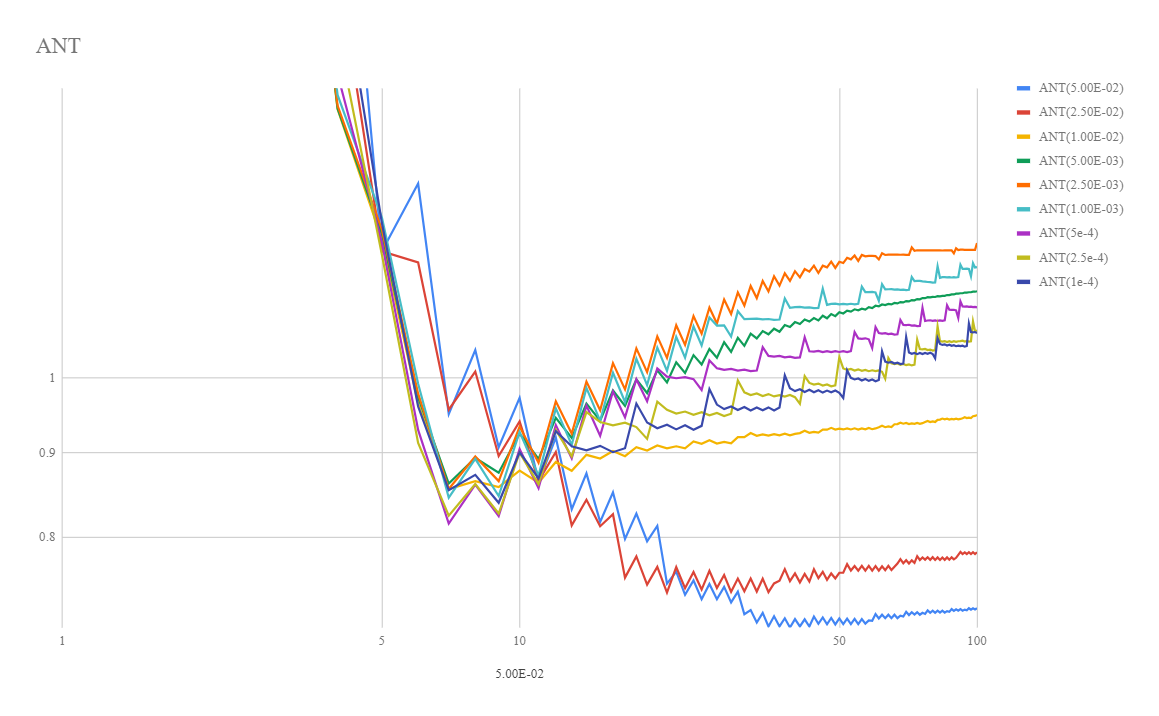
\includegraphics[width=\textwidth]{{figures/ml1m_ant_valoss_iter_lambda.png}}
                \caption{Ant}
        \end{subfigure}
        \begin{subfigure}[b]{0.9\textwidth}
                \centering
                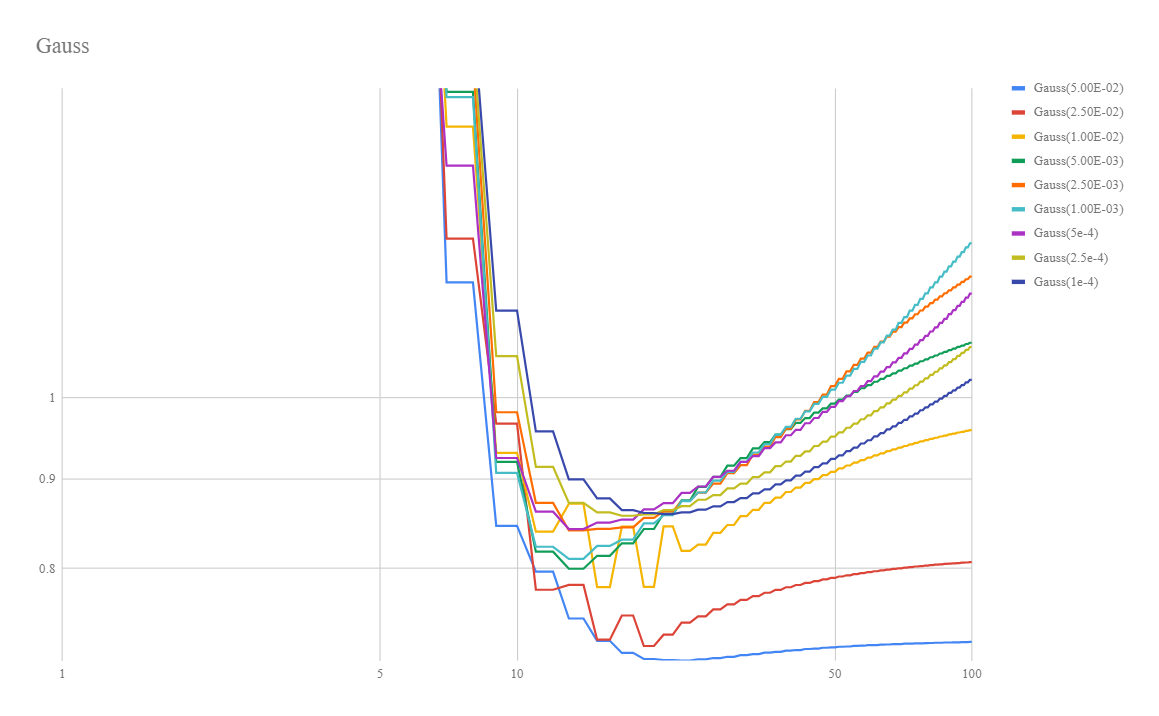
\includegraphics[width=\textwidth]{{figures/ml1m_gauss_valoss_iter_lambda.png}}
                \caption{Gauss}
        \end{subfigure}
        \caption{ml-1m. A comparison on the va-loss of different $\lambda$. 
        The $x$-axis is the iteration,
        while the $y$-axis is the va-loss.}\label{fig:ml1m_ant_gauss_valoss_iter_lambda}
\end{figure*}

\begin{figure*}[tb]
        \centering
        \begin{subfigure}[b]{0.9\textwidth}
                \centering
                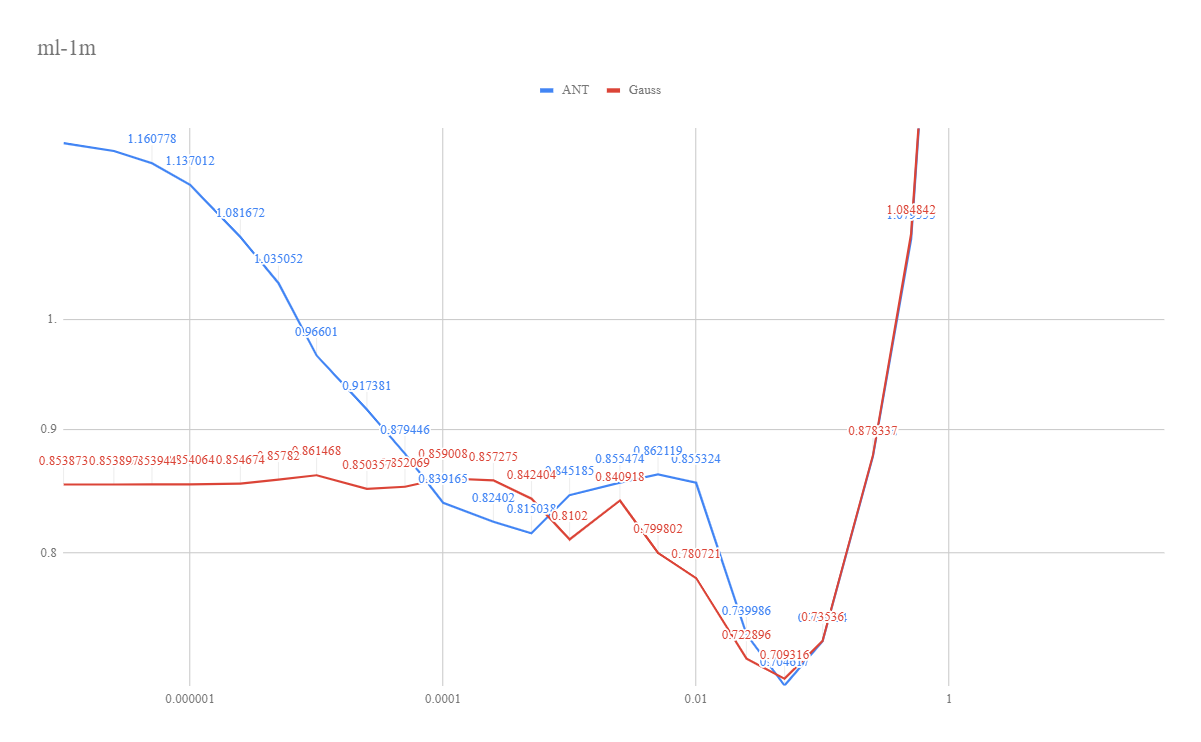
\includegraphics[width=\textwidth]{{figures/ml1m_valoss_lambda.png}}
%                \caption{Ant}
        \end{subfigure}        
        \caption{ml-1m. A comparison on the best va-loss of different methods.
        The $x$-axis is $\lambda$,
        while the $y$-axis is the va-loss.}\label{fig:ml1m_ant_gauss_valoss_lambda}
\end{figure*}